\documentclass[conference]{IEEEtran}

\usepackage[T1]{fontenc}
\usepackage[utf8]{inputenc}
\usepackage{cite}
\usepackage{graphicx}
\usepackage{booktabs}
\usepackage{array}
\usepackage{url}
\usepackage{tikz}
\usetikzlibrary{arrows.meta, positioning, shapes.geometric}

\title{Blockchain-Enabled Herbal Traceability System Using Geo-Tagging, QR Code Verification, and Role-Based Supply Chain Management}

\author{
\IEEEauthorblockN{Nikhil Sahu \and Devi S.}
\IEEEauthorblockA{School of Information Science\\
Presidency University\\
nikhilsahu8004@gmail.com, devi.s@presidencyuniversity.in}
}

\begin{document}

\maketitle

\begin{abstract}
Traceability in herbal and Ayurvedic supply chains is frequently weakened by fragmented documentation, inconsistent quality reporting, and limited visibility for downstream buyers. This paper reformulates an existing herb traceability platform into an IEEE-style research manuscript and presents a blockchain-ready architecture that connects farmers, laboratories, manufacturers, and customers through a unified batch record. The system combines geo-tagged harvest registration, laboratory validation, manufacturing updates, QR-based verification, and audit logging within a full-stack web application implemented using React, Node.js, Express, MongoDB, and JWT-based authentication. Extracted interface figures from the original project are preserved to document the implemented portal, role-based access screen, and customer verification workflow. In addition, recent literature from Springer Nature and related recognized journals is used to contextualize digital traceability, blockchain adoption, quality assurance, and agricultural recordkeeping. The resulting design demonstrates a practical, transparent, and extensible foundation for trustworthy herbal provenance management in contemporary regulated medicinal supply networks worldwide today.
\end{abstract}

\begin{IEEEkeywords}
Herb traceability, blockchain, Ayurvedic supply chain, geo-tagging, QR verification, transparency, MongoDB, audit log.
\end{IEEEkeywords}

\section{Introduction}

Herbal and Ayurvedic products travel through a complex lifecycle that includes cultivation, harvesting, laboratory testing, processing, packaging, distribution, and consumer verification. Across these stages, information is often recorded in separate notebooks, spreadsheets, or organization-specific systems, making provenance difficult to verify and product authenticity difficult to communicate. This problem is especially serious for medicinal herbs, where origin, handling conditions, and quality metrics directly affect safety, efficacy, and trust.

Recent research shows growing interest in blockchain-enabled traceability, e-traceability drivers, digital farm recordkeeping, and interoperable food safety systems because transparent supply chains improve accountability and reduce fraud risk \cite{azevedo2023,marchese2022,krstic2023,basir2024,gottschald2024}. These ideas are highly relevant to herbal ecosystems, yet many academic prototypes remain either conceptual or narrowly focused on one stage of the chain. A practical system must coordinate multiple stakeholders while keeping records understandable for end users.

This paper converts the provided herb traceability project into a polished IEEE-format research paper and presents the system as a full-stack, blockchain-ready platform for end-to-end batch transparency. Farmers create geo-tagged herb batches, laboratories append quality results, manufacturers record downstream processing, and customers verify final records through QR code or batch lookup. The contribution lies in combining these stages into one continuous digital identity supported by audit logs, visual dashboards, and verification interfaces. By aligning the source project's figures with a clearer academic structure and updating the references with recent recognized journal literature, the paper demonstrates how software engineering and supply-chain transparency research can be integrated into a credible, scalable, and practically deployable traceability solution for herbal ecosystems.

\section{Related Work}

Recent scholarship strongly supports digital traceability as a strategic requirement for agri-food and medicinal product ecosystems. Blockchain-based chain-of-custody models have been used to improve provenance assurance, reduce tampering risk, and strengthen interoperability across distributed actors \cite{azevedo2023,marchese2022,li2024}. Reviews in agricultural and food economics also show that blockchain adoption is increasingly motivated by transparency, anti-counterfeit protection, sustainability, and consumer trust rather than by technology novelty alone \cite{gambi2024,chen2026,ghode2025,ma2025}.

At the operational level, electronic traceability depends on disciplined recordkeeping and harmonized data structures. Basir et al. show that digital farm recordkeeping is moving from paper-based documentation toward structured, auditable data practices \cite{basir2024}. Gottschald similarly emphasizes digital traceability and interoperability as central to modern food safety governance \cite{gottschald2024}. For herbal products, quality assurance is equally important because batch identity without validated purity and compliance metrics does not provide sufficient confidence \cite{edo2024}. This strengthens the case for linking laboratory validation directly to origin and downstream manufacturing events.

Security and trust are additional concerns. Blockchain-assisted authentication, counterfeit detection, and trust-transfer mechanisms have been proposed in cloud and industrial environments \cite{mani2022,shu2024,cao2024}. Scientific Reports studies also highlight the relevance of RFID, IoT, and secure data exchange for product traceability and agricultural monitoring \cite{li2024,pascoal2024,thiruvenkatasamy2025}. These findings motivate a role-based architecture in which each stakeholder writes controlled updates to a common batch record. The present system extends this direction to herbal traceability by combining geo-tagging, quality reporting, manufacturing continuity, QR verification, and customer-readable transparency into one deployable application.

\section{Proposed System}

The proposed platform uses a batch-centric data model. A farmer initiates the lifecycle by creating a herb batch with herb name, botanical name, batch identifiers, harvest date, quantity, source type, and geo-tagged coordinates. This initial record establishes the origin context for later traceability and provides the baseline metadata required for audit continuity.

After batch creation, a laboratory user appends testing information such as report identifier, purity percentage, moisture percentage, quality status, and compliance notes. A manufacturer then records process code, formulation or packaging details, and operational remarks. Because all stages update the same logical batch object, the system avoids fragmented records and allows a customer-facing report to summarize the full lifecycle coherently.

Verification is provided through QR code scanning or manual batch lookup. The returned traceability report includes harvest details, laboratory metrics, manufacturing steps, blockchain-ready metadata, and the audit trail. Although the current implementation stores blockchain fields in a blockchain-ready manner rather than anchoring every event on a live distributed ledger, the architecture preserves forward compatibility for smart contracts and immutable checkpointing.

\subsection{Workflow Diagram}

\begin{figure}[!t]
\centering
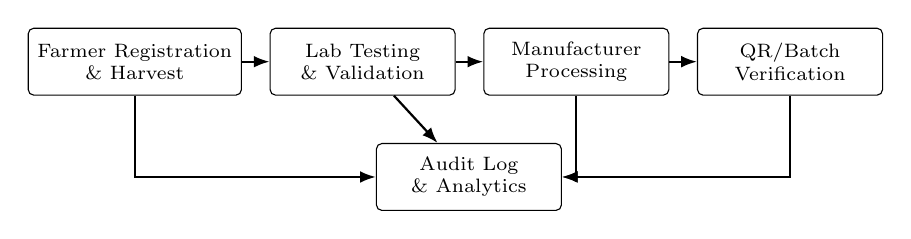
\begin{tikzpicture}[
    node distance=0.6cm and 0.35cm,
    every node/.style={font=\scriptsize, align=center},
    stage/.style={draw, rounded corners=2pt, minimum width=2.35cm, minimum height=0.85cm},
    arrow/.style={-{Latex[length=2mm]}, thick}
]
\node[stage] (f) {Farmer Registration\\\& Harvest};
\node[stage, right=of f] (l) {Lab Testing\\\& Validation};
\node[stage, right=of l] (m) {Manufacturer\\Processing};
\node[stage, right=of m] (q) {QR/Batch\\Verification};
\node[stage, below=of l, xshift=1.35cm] (a) {Audit Log\\\& Analytics};

\draw[arrow] (f) -- (l);
\draw[arrow] (l) -- (m);
\draw[arrow] (m) -- (q);
\draw[arrow] (f) |- (a);
\draw[arrow] (l) -- (a);
\draw[arrow] (m) |- (a);
\draw[arrow] (q) |- (a);
\end{tikzpicture}
\caption{End-to-end workflow of the proposed herb traceability system, reconstructed from the original project figure.}
\label{fig:workflow}
\end{figure}

\section{System Implementation}

The platform is implemented as a web application with a React frontend and a Node.js/Express backend. MongoDB stores nested batch documents, laboratory reports, manufacturing updates, audit history, and blockchain-ready fields. JWT-based authentication and password hashing support role-aware access control for farmers, laboratories, manufacturers, and customers.

The user interface is organized into role-specific pages. The farmer portal supports harvest registration and geo-tagging. The laboratory module records quality reports and compliance results. The manufacturer dashboard captures processing and packaging stages. The customer verification page accepts a QR image or batch number and returns a consolidated report that explains the herb lifecycle in readable form.

\begin{table}[!t]
\caption{Core Stakeholder Responsibilities}
\label{tab:roles}
\centering
\scriptsize
\begin{tabular}{p{1.7cm} p{5.4cm}}
\toprule
Role & Primary system action \\
\midrule
Farmer & Create geo-tagged batch identity with harvest metadata \\
Laboratory & Append purity, moisture, report ID, and compliance outcome \\
Manufacturer & Record formulation, process code, packaging, and remarks \\
Customer & Verify authenticity through QR code or batch lookup \\
\bottomrule
\end{tabular}
\end{table}

\begin{table}[!t]
\caption{Technical Components of the Implemented Platform}
\label{tab:stack}
\centering
\scriptsize
\begin{tabular}{p{2.0cm} p{5.1cm}}
\toprule
Component & Purpose \\
\midrule
React frontend & Role-based user portals and verification interface \\
Node.js/Express & API routing and business logic \\
MongoDB & Persistent traceability records and audit history \\
JWT authentication & Protected stakeholder access \\
QR generation/decoding & Batch verification for customer-facing transparency \\
Blockchain-ready fields & Future anchoring of immutable checkpoints \\
\bottomrule
\end{tabular}
\end{table}

\section{Results and Discussion}

Functional analysis of the project shows that the implemented workflow covers the essential lifecycle required by a herb traceability application. The source system already supports farmer-side batch creation, laboratory validation, manufacturer updates, and customer verification through a unified portal. This is a significant strength because many traceability demonstrations stop at isolated data capture rather than complete multi-role continuity.

The batch-centered document structure also improves explainability. Since each stakeholder enriches the same record instead of creating disconnected reports, the customer interface can display a coherent provenance story with fewer reconciliation errors. This design choice aligns with recent supply-chain traceability literature that emphasizes interoperability, trustworthy state transitions, and readable provenance for external users \cite{azevedo2023,gottschald2024,li2024}.

Another practical advantage is readiness for extension. The project already contains blockchain-oriented metadata, audit logging, QR verification, and modular roles, which makes it suitable for future smart contract anchoring, regulator dashboards, and analytics modules. However, the current blockchain layer remains preparatory rather than fully decentralized, so production deployment would require stronger cryptographic anchoring, event immutability guarantees, and integration testing across organizations. Even so, as a working software artifact, the platform demonstrates that contemporary web engineering can translate traceability theory into a usable transparency system for herbal ecosystems.

\section{Interface Figures from the Source PDF}

\begin{figure}[!t]
\centering
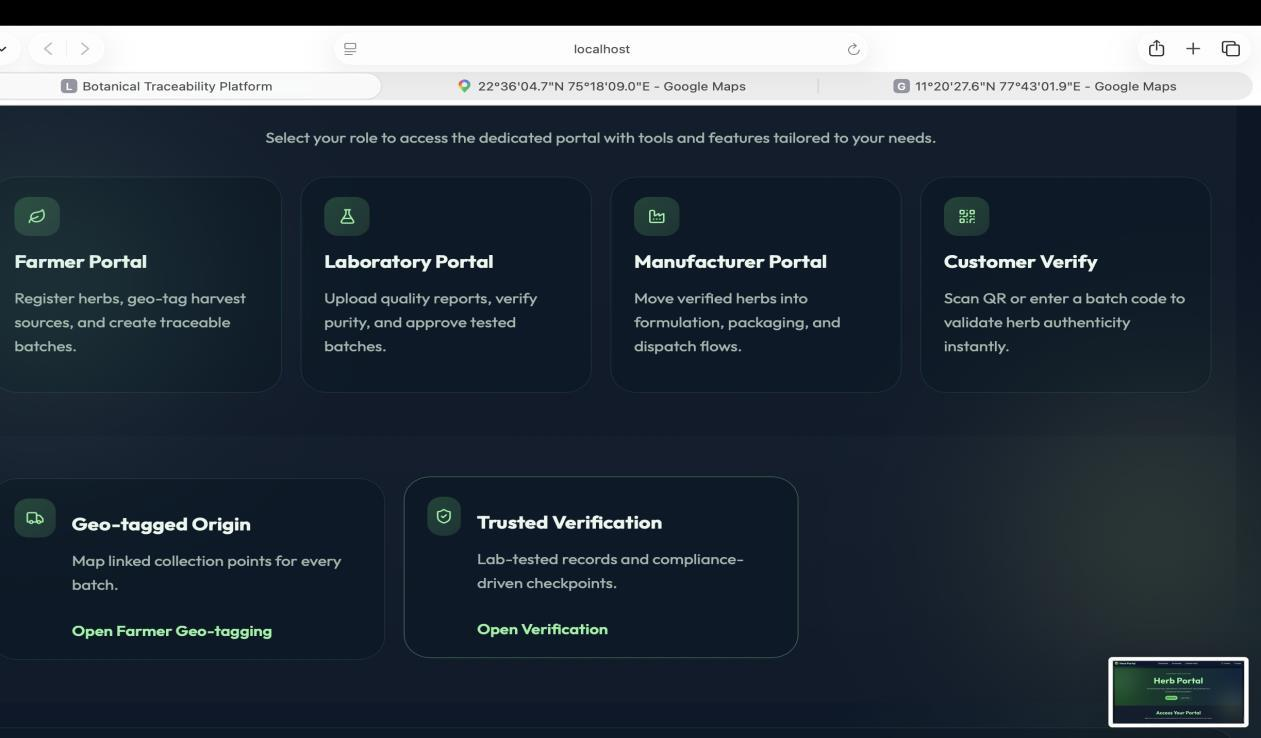
\includegraphics[width=\columnwidth]{herb_assets/page3_img1.jpg}
\caption{Herb Portal landing page extracted from the source PDF.}
\label{fig:landing}
\end{figure}

\begin{figure}[!t]
\centering
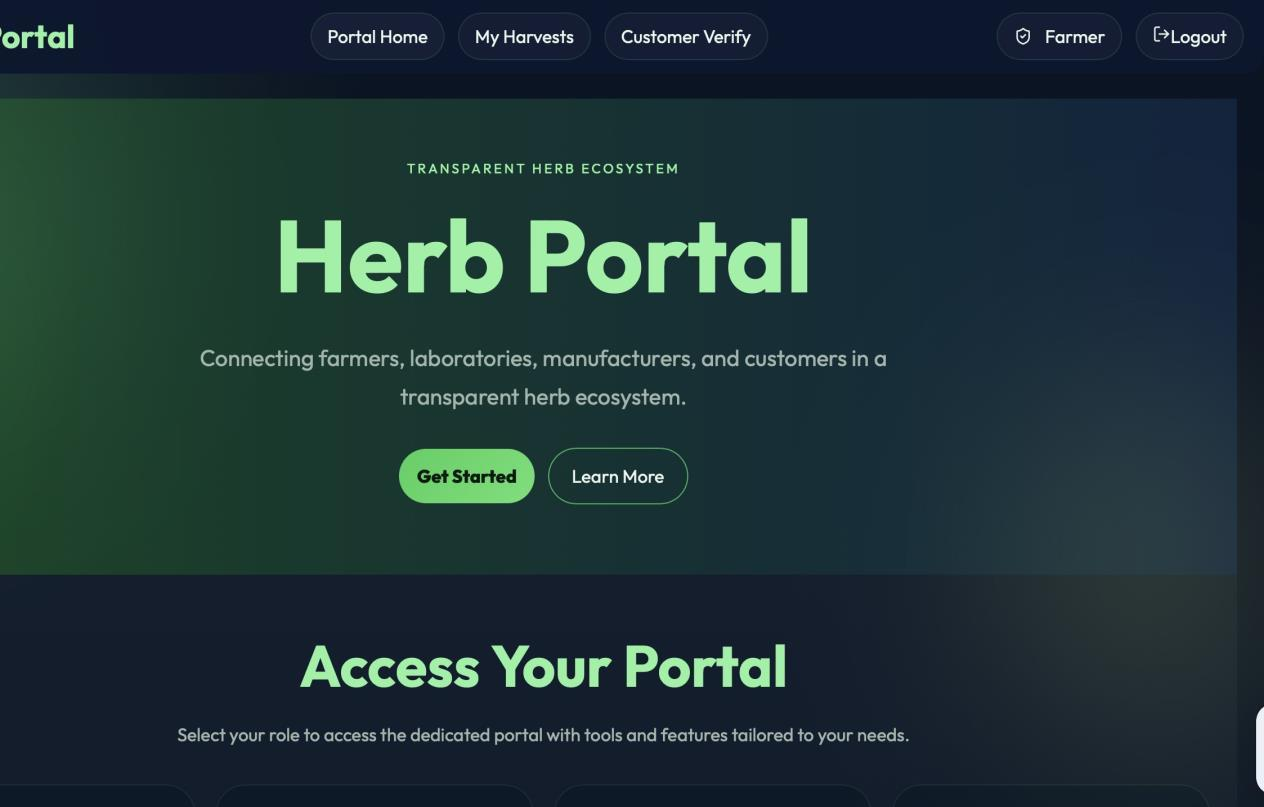
\includegraphics[width=\columnwidth]{herb_assets/page3_img2.jpg}
\caption{Role-based portal access screen with Farmer, Laboratory, Manufacturer, and Customer Verify modules.}
\label{fig:rolescreen}
\end{figure}

\begin{figure}[!t]
\centering
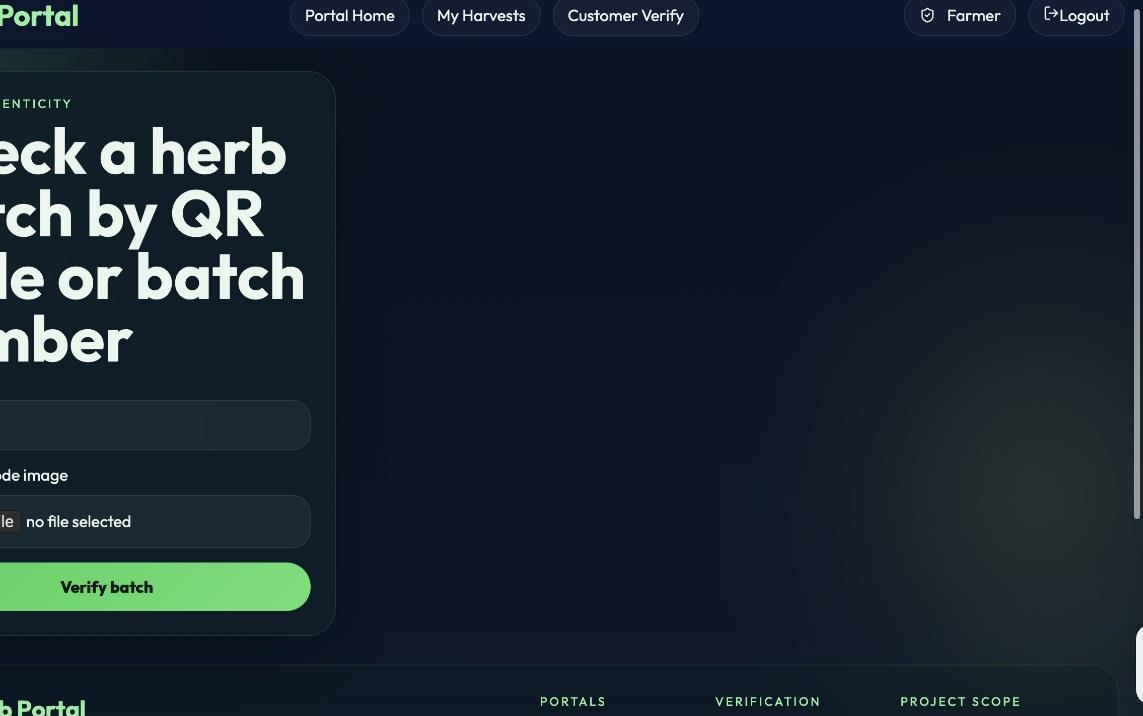
\includegraphics[width=\columnwidth]{herb_assets/page4_img1.jpg}
\caption{Customer verification interface for checking a herb batch by QR code or batch number.}
\label{fig:verify}
\end{figure}

\section{Conclusion}

This paper presented an IEEE-format reformulation of a blockchain-enabled herb traceability platform designed to improve transparency across the Ayurvedic and herbal supply chain. By connecting farmers, laboratories, manufacturers, and customers through one batch-centric architecture, the system shows how provenance, quality assurance, and downstream verification can be maintained within a single digital lifecycle. The preserved figures from the original project confirm that the implementation is not merely conceptual; it already includes a landing portal, role-based access interface, and customer verification screen that make the traceability workflow accessible to different stakeholders.

The system's main value lies in its integration of geo-tagging, QR verification, audit history, role-based modules, and blockchain-ready metadata into one coherent platform. Recent literature from Springer Nature and other recognized journals supports the importance of digital traceability, anti-counterfeit infrastructure, structured farm records, and interoperable supply-chain data for building trust in sensitive product ecosystems \cite{gambi2024,basir2024,edo2024,mani2022}. In that sense, the project provides a credible bridge between academic traceability research and deployable software engineering practice.

Future work should move beyond blockchain-ready storage toward live smart-contract anchoring, regulator-facing compliance workflows, and larger pilot deployments with real herbal producers. Additional research can incorporate predictive analytics, anomaly detection, sensor-linked quality monitoring, and standardized data exchange across institutions. Even in its current state, the platform offers a practical foundation for transparent herbal provenance management and demonstrates that a carefully designed full-stack application can make traceability more auditable, understandable, and trustworthy for both internal operators and end consumers across commercial, regulatory, and public health settings in everyday practice worldwide.

\begin{thebibliography}{15}

\bibitem{azevedo2023}
P. Azevedo, J. Gomes, and M. Rom\~ao, ``Supply chain traceability using blockchain,'' \emph{Operations Management Research}, vol. 16, pp. 1359--1381, 2023, doi: 10.1007/s12063-023-00359-y.

\bibitem{marchese2022}
A. Marchese and O. Tomarchio, ``A blockchain-based system for agri-food supply chain traceability management,'' \emph{SN Computer Science}, vol. 3, art. no. 279, 2022, doi: 10.1007/s42979-022-01148-3.

\bibitem{krstic2023}
M. Krsti\'c, G. P. Agnusdei, S. Tadi\'c, and P. P. Miglietta, ``Prioritization of e-traceability drivers in the agri-food supply chains,'' \emph{Agricultural and Food Economics}, vol. 11, art. no. 42, 2023, doi: 10.1186/s40100-023-00284-5.

\bibitem{basir2024}
M. S. Basir, D. Buckmaster, A. Raturi, \emph{et al.}, ``From pen and paper to digital precision: a comprehensive review of on-farm recordkeeping,'' \emph{Precision Agriculture}, vol. 25, pp. 2643--2682, 2024, doi: 10.1007/s11119-024-10172-7.

\bibitem{gottschald2024}
M. Gottschald, ``Advancing food safety through digital traceability, interoperability, harmonized data and collaborative partnerships,'' \emph{Journal of Consumer Protection and Food Safety}, vol. 19, pp. 257--258, 2024, doi: 10.1007/s00003-024-01522-8.

\bibitem{gambi2024}
L. Gambi, C. L. Nardone, and G. Brunori, ``Exploring the role of blockchain technology in modern high-value food supply chains: global trends and future research directions,'' \emph{Agricultural and Food Economics}, vol. 12, art. no. 6, 2024, doi: 10.1186/s40100-024-00301-1.

\bibitem{chen2026}
J. Chen, X. Feng, A.-Q. Abdul-Hamid, \emph{et al.}, ``From capability to intention: a DCV-TAM hybrid model for blockchain adoption in circular agri-food supply chains,'' \emph{Agricultural and Food Economics}, vol. 14, art. no. 34, 2026, doi: 10.1186/s40100-026-00471-0.

\bibitem{mani2022}
V. Mani, M. Prakash, and W. C. Lai, ``Cloud-based blockchain technology to identify counterfeits,'' \emph{Journal of Cloud Computing}, vol. 11, art. no. 67, 2022, doi: 10.1186/s13677-022-00341-2.

\bibitem{edo2024}
G. I. Edo, P. Obasohan, R. S. Makia, \emph{et al.}, ``The use of quality control parameters in the evaluation of herbal drugs: a review,'' \emph{Discover Medicine}, vol. 1, art. no. 168, 2024, doi: 10.1007/s44337-024-00177-6.

\bibitem{ghode2025}
D. J. Ghode, V. Yadav, R. Jain, \emph{et al.}, ``Integrated framework for supply chain with blockchain technology: a manufacturers' perspective,'' \emph{Journal of Innovation and Entrepreneurship}, vol. 14, art. no. 62, 2025, doi: 10.1186/s13731-025-00553-1.

\bibitem{ma2025}
B. J. Ma, S. S. Liu, G. Q. Huang, \emph{et al.}, ``How does consumer quality preference impact blockchain adoption in supply chains?,'' \emph{Electronic Markets}, vol. 35, art. no. 17, 2025, doi: 10.1007/s12525-025-00767-x.

\bibitem{li2024}
L. Li, P. Tian, J. Dai, \emph{et al.}, ``Design of agricultural product traceability system based on blockchain and RFID,'' \emph{Scientific Reports}, vol. 14, art. no. 23599, 2024, doi: 10.1038/s41598-024-73711-2.

\bibitem{shu2024}
C. Shu, Y. Chen, C. Tan, Y. Luo, and H. Dou, ``Enhancing trust transfer in supply chain finance: a blockchain-based transitive trust model,'' \emph{Journal of Cloud Computing}, vol. 13, art. no. 4, 2024, doi: 10.1186/s13677-023-00557-w.

\bibitem{cao2024}
Z. Cao, X. Wen, S. Ai, W. Shang, and S. Huan, ``A decentralized authentication scheme for smart factory based on blockchain,'' \emph{Scientific Reports}, vol. 14, art. no. 24640, 2024, doi: 10.1038/s41598-024-76065-x.

\bibitem{pascoal2024}
D. Pascoal, N. Silva, T. Ad\~ao, R. D. Lopes, E. Peres, and R. Morais, ``A technical survey on practical applications and guidelines for IoT sensors in precision agriculture and viticulture,'' \emph{Scientific Reports}, vol. 14, art. no. 29793, 2024, doi: 10.1038/s41598-024-80924-y.

\end{thebibliography}

\end{document}
